\documentclass[11pt,a4paper]{article}
\usepackage[utf8]{inputenc}
\usepackage[hmargin=2.0cm,vmargin=2.5cm,bindingoffset=0.5cm]{geometry}
\usepackage{amsfonts}
\usepackage{amsmath,amsthm,amssymb}
\allowdisplaybreaks
\usepackage{hyperref}
\usepackage{graphicx}
\usepackage{tikz}
\usepackage{mathtools}
\DeclarePairedDelimiter\ceil{\lceil}{\rceil}
\DeclarePairedDelimiter\floor{\lfloor}{\rfloor}
%\usepackage{float}
\usepackage{placeins}
\usepackage{diagbox}
\DeclareMathOperator{\Tr}{Tr}
\newtheorem{thm}{Theorem}
\usepackage{subcaption}
%\usepackage{subfigure}
\usepackage[english]{babel}
\author{Mohit}
\title{Adiabatic gauge potential of quantum integrable and non-integrable systems  }
\begin{document}
\maketitle
%\tableofcontents

\section{Introduction}

Adiabatic gauge potentials are useful for controlling a quantum system when it's driven externally from one configuration to another. These potentials help us in  circumventing standard adiabatic limitations which requires infinitesimally small rates \cite{demirplak2003adiabatic,demirplak2005assisted, berry2009transitionless}. For example, these potentials can be used for arbitrarily fast annealing protocols and implementing fast dissipationless driving. 



The scaling of norm of gauge potential with system's size is quite different for  quantum integrable and non-integrable systems. On one hand, for integrable systems , exact gauge potential are supposed to scale like a polynomial in system size. This is due to extensive number of symmetries that exist and as a result, they have a ``lot" of degenerate energy levels which comes with their respective ``selection rules".  This can be easily seen  for Transverse Ising model whose analytical expression of gauge potential is known in literature.

On the other hand, for non-integrable systems, using  Eigenstate Thermalization Hypothesis (ETH)\cite{d2016quantum} , we can show that norm of exact gauge potential scale exponentially in system size. This can be verified numerically using exact diagonalization on spin system upto size $L=15$. 


We can exploit this property to distinguish  between quantum integrable and non-integrable system. Our method should be better than conventional method (energy level distribution) used in literature for this purpose because unlike the conventional method, we don't have to worry about removing symmetry.


%The goal, as of now, is to distinguish between integrable and non-integrable many-body quantum system by studying their approximate gauge adiabatic potential\footnote{We expect results to be valid for classical system too. But for now, we would focus on quantum systems.}

 



\section{Adiabatic gauge potential}
\subsection{Introduction by example}


\begin{equation}
H_0= \dfrac{p^2}{2m} + V(x- \lambda(t))
\end{equation}

\begin{align*}
H_{CD}= H_0 + \dot{\lambda} A_{\lambda}
\end{align*}
where $A_{\lambda}= p$.
Include a picture of glass of water being transported from Dries's PNAS paper. Question: if you have exact gauge potential, does all the excitations during intermediate times is zero.

\subsection{Formal introduction}
Adiabatic gauge potentials are the generators of a unitary transformation which diagonalize the instantaneous Hamiltonian, attempting to leave its eigenbasis invariant as the parameter is changed. These adiabatic gauge potentials generate \textit{non-adiabatic} corrections to Hamiltonian in the moving basis ($\lambda$ -dependent basis).
 
 This is something from Anatoli's lecture notes \cite{kolodrubetz2016geometry}--
``an adiabatic basis is a family of adiabatically connected eigenstates, i.e., eigenstates related
to a particular initial basis by adiabatic (infinitesimally slow) evolution of the parameter $\lambda$. For example, if two levels cross they will exchange order energetically but the adiabatic connection will be non-singular."


$H (\lambda) |n(\lambda) \rangle = E_n (\lambda) |n(\lambda) $. Let's derive diagonal and off-diagonal elements. 


\begin{itemize}
\item \textbf{n-th diagonal element:} $A_{\lambda}^n= \langle n |A_{\lambda} | n \rangle=  i \hbar\langle n |\partial_{\lambda} | n \rangle $
\item \textbf{off- diagonal element:} We use the identity $\langle m |H(\lambda) | n \rangle=0 \quad, n \neq m$ and then differentiate with respect to $\lambda$ to obtain:
\begin{align}
\boxed{\langle m |A_{\lambda} | n \rangle =  -i \hbar \dfrac{\langle m |\partial_{\lambda}H | n \rangle}{E_m-E_n}}
\end{align}
where both  energies ($E_m, E_n$) and eigenvectors ($|m \rangle, |n \rangle$) depend on $\lambda$.
\end{itemize}







\subsection{Eigenstate Thermalization Hypothesis}
Eigenstate Thermalization Hypothesis( ETH) gives us an ansatz for matrix elements of observables in the basis of energy eigenstates  \cite{d2016quantum}:
\begin{equation}
O_{mn}= O( \bar{E}) \delta_{mn} + e^{-S(\bar{E})/2} f_O(\bar{E}, \omega) R_{mn}
\end{equation}
where $\bar{E}= (E_m +E_n)/2, \omega= E_n- E_m$ and $S(E)$ is the thermodynamic entropy at energy $E$.

We note that it's applicable only for few-body operators of a non-integrable Hamiltonian. By few-body, we mean $n$ body observables with $n \ll N$, where $N$ is the total number of spins, particles, etc. For example, projection operator to eigenstates of many body  Hamiltonian $\hat{P}_{\alpha}= |\Psi_{\alpha} \rangle \langle\Psi_{\alpha}  |$ don't satisfy ETH and it also doesn't satisfy predictions of statistical mechanics. Why is that? We expect that microcanonical averaging should be equivalent to canonical averaging:
\begin{equation}
 \langle\Psi_{\alpha}  |O|\Psi_{\alpha} \rangle= \dfrac{\Tr O e^{-\beta H}}{\Tr e^{-\beta H}}
\end{equation}
We can see $O= \hat{P}_{\alpha}$ doesn't satisfy the above equation (since left hand side is one and the trace of right hand side can be computed in energy basis to find that it's not one). Projection operator is non-local in real space, and we argue that this is the reason it doesn't satisfy ETH and is not experimentally measurable.

\subsubsection{Information about $f_O(\bar{E}, \omega)$}

\begin{equation}
 |f_O(\bar{E}, \omega)|=\left\{
  \begin{array}{@{}ll@{}}
    e^{-\omega T} & (\omega \gg T), \\
     \dfrac{\sqrt{L}}{\omega^2+ \mu_T^2} & (\omega \ll T)
  \end{array}\right.
\end{equation}
where $\mu_T^2 \sim \dfrac{1}{L^2}$ \cite{khatami2013fluctuation, srednicki1999approach,d2016quantum}
\section{Norm of adiabatic gauge potential}
Let's compute the norm by noting that $A_{\lambda}$ has only off-diagonal elements in energy basis in our gauge choice:

\begin{align}
||A_{\lambda}||^2 &= \Tr  A_{\lambda}^2 \\
&= \sum_n \langle n | A^2_{\lambda}| n \rangle \\
&= \sum_{n} \langle n | A_{\lambda}| n \rangle ^2 + \sum_n \sum_{m \neq n}  |\langle m | A_{\lambda}| n \rangle|^2 \\
&=  \sum_n \sum_{m \neq n}  |\langle m | A_{\lambda}| n \rangle|^2 \\
&= \hbar^2 \sum_n \sum_{m \neq n}  \dfrac{|\langle m | \partial_{\lambda}H| n \rangle|^2}{(E_m-E_n)^2} 
\end{align}

Hence, in general, for both integrable and non-integrable systems we have: 
\begin{equation}
\boxed{||A_{\lambda}||^2 = \hbar^2\sum_n \sum_{m \neq n}  \dfrac{|\langle m | \partial_{\lambda}H| n \rangle|^2}{(E_m-E_n)^2} }
\end{equation}


\section{Integrable model}
Our goal is to study a integrable model, which is called \textbf{Transverse Field Ising model}. It shows quantum phase transition between ferromagnetic and paramagnetic phases. Moreover, it satisfies Ising symmetry $G= \Pi_i \sigma_i^z$ since $[H, G]=0$, where $H$ is the Hamiltonian.
This model can be written in terms of non-interacting spinless fermions ($c_i, c^{\dagger}_i $) using Jordan- Wigner transformation. 

It's Hamiltonian in spin basis is given by:
\begin{equation}
H= -J \sum_{j=1}^{L} \sigma_j^x \sigma_{j+1}^x - \lambda \sum_{j} \sigma_j^z 
\label{xx_z}
\end{equation}
where we have chosen periodic boundary conditions and $\lambda$ is externally-controlled transverse magnetic field.

This model can be written in terms of non-interacting spinless fermions ($c_i, c^{\dagger}_i $) using Jordan- Wigner transformation: $\sigma_i^z \sim 1 - 2 c^{\dagger}_i c_i   $ and $\sigma_i^+ \sim \prod_{j<i} \sigma_j^z c_j   $. Details can be found elsewhere \cite{sachdev2007quantum} \footnote{Momentum operator chosen to get real valued Hamiltonian is $c_k= \frac{e^{i \pi/4}}{\sqrt{L}}\sum_j c_j e^{-ikj}$, where k is $n\pi/L$ with $n=0,1,2, \ldots L-1$} . Here is what we get after this transformation:

\begin{equation}
\mathcal{H}= \sum_k \psi_k^{\dagger} H_k \psi_k , \quad H_k=-\begin{bmatrix}
     \lambda - \cos k & \sin k \\
\sin k & -(\lambda - \cos k)\\
\end{bmatrix}
\end{equation}
where $\psi_k^{\dagger}= (c^{\dagger}_k, c_{-k})$ is Nambu spinor basis. We can write $H_k$ in terms of Pauli sigma matrices:
\begin{equation}
H_k= -(\lambda - \cos k) \sigma^z_k - \sin k  \sigma^x_k
\end{equation}



Now using our regulator method (whose details are not given in this report), we can obtain :
\begin{equation}
\boxed{A_{\lambda}= \sum_{l=1}^{L-1} \alpha_l O_l \quad \mbox{where} \quad \alpha_l= -\dfrac{1}{4 L} \sum_k \dfrac{\sin(k) \sin(lk)}{(\cos k - \lambda)^2 + \sin^2 k}}
\end{equation}
where  $O_l$ is given by
\begin{equation}
O_l= 2 i \sum_j (c^{\dagger}_{j} c^{\dagger}_{j+l} - \mbox{h.c})= \sum_j ( \sigma_j^x \sigma_{j+1}^z \ldots \sigma_{j+l-1}^z \sigma_{j+l}^y +  \sigma_j^y \sigma_{j+1}^z \ldots \sigma_{j+l-1}^z \sigma_{j+l}^x)
\end{equation}
This matches with the result already known in literature \cite{del2012assisted, kolodrubetz2016geometry}.


Let's write a first few terms of $O_l$ here:
\begin{align*}
O_{l=1}&=  \sum_{j=1}^{L} ( \sigma_j^x  \sigma_{j+1}^y +  \sigma_j^y  \sigma_{j+1}^x) \\
O_{l=2} &=  \sum_{j=1}^{L} ( \sigma_j^x \sigma_{j+1}^z \sigma_{j+2}^y +  \sigma_j^y \sigma_{j+1}^z \sigma_{j+2}^x) 
\end{align*}

On computation, we find that with periodic boundary conditions, we get $\Tr O_l  O_p= \delta_{l,p} 2^{L+1} L$

For large enough system size $L$, we can compute $\alpha_l$ \cite{kolodrubetz2016geometry} by computing the sum into an integral and obtain the value of $\alpha_l$ as: 
\begin{equation}
 \alpha_l=-\dfrac{1}{8}\left\{
  \begin{array}{@{}ll@{}}
    \lambda^{l-1} & (\lambda^2 <1), \\
     \lambda^{-l-1} & (\lambda^2 >1)
  \end{array}\right.
\end{equation}




\begin{figure}[!ht]
\begin{center}
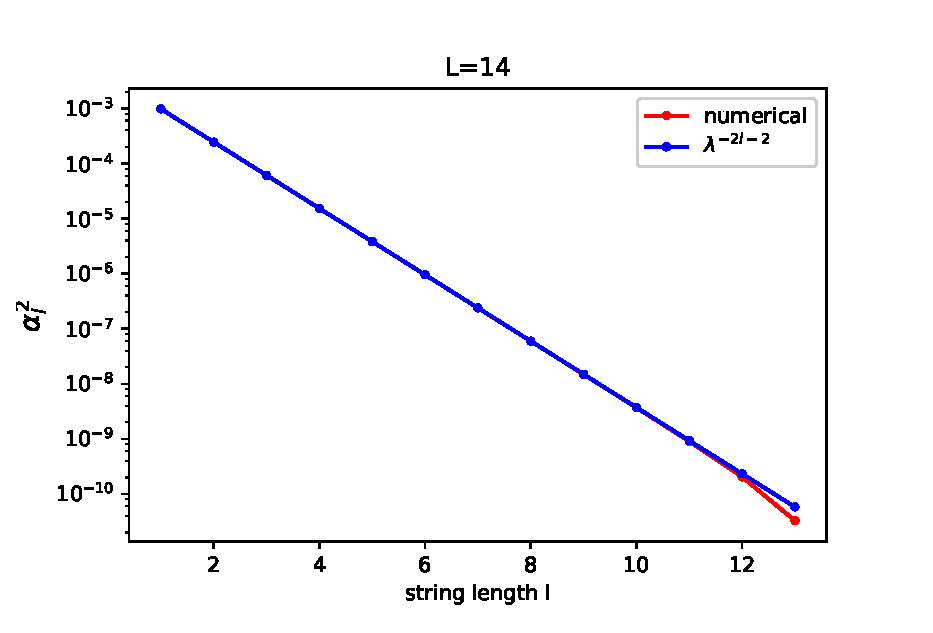
\includegraphics[scale=0.7]{new_pics/alpha_num_theoret.eps}\\
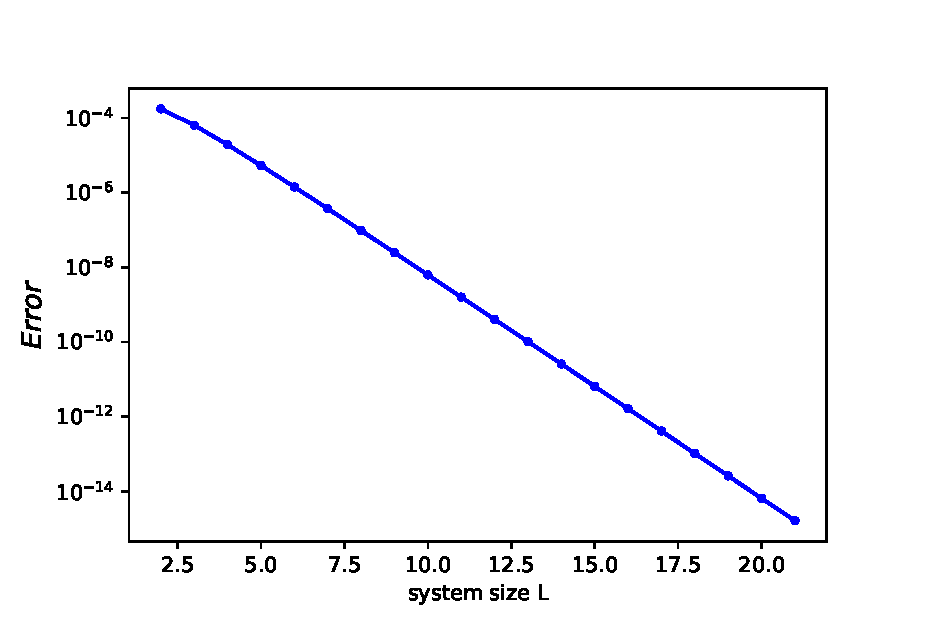
\includegraphics[scale=0.7]{new_pics/error_alpha.eps}\\
\caption{Integrable systems: string length of exact gauge potential as a function of system size }
\end{center}
\end{figure}

Let's compute norm of gauge potential:
\begin{align}
||A_{\lambda}||^2 &= \Tr  A_{\lambda}^2 \\
&= \Tr \sum_{l,p}  \alpha_p \alpha_l O_l  O_p\\
&=  \sum_{l,p}  \alpha_p \alpha_l  \Tr O_l  O_p\\
&=  2^{L+1} L \sum_{l=1}^{L-1}   \alpha_l ^2
\end{align}

\begin{figure}[!ht]
\begin{center}
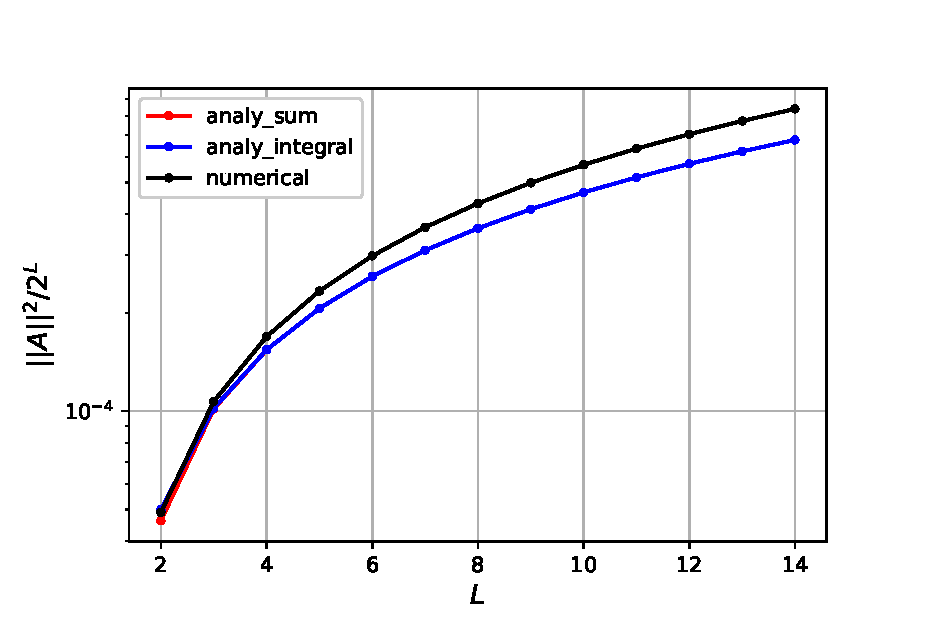
\includegraphics[scale=0.7]{new_pics/OBC_int_comparing_num_anal_norm_L_scaling.eps}
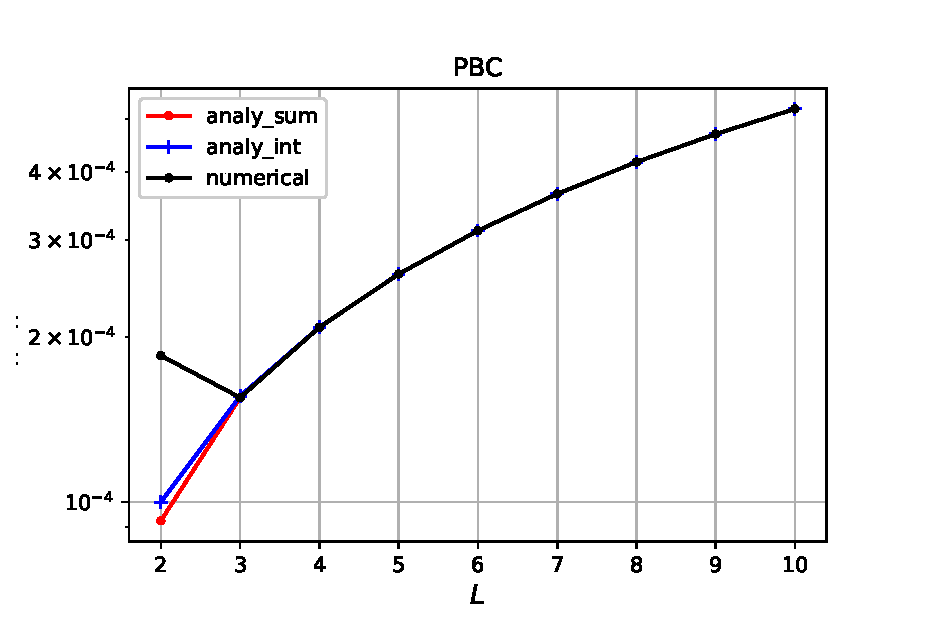
\includegraphics[scale=0.7]{new_pics/PBC_int_comparing_num_anal_norm_L_scaling.eps}
\caption{Integrable systems: Norm of exact gauge potential as a function of system size }
\end{center}
\end{figure}



Now since $\alpha_l$ for large enough $L$ is exponentially suppressed in $l$, we can argue that


\begin{equation}
\boxed{||A_{\lambda}||^2 / 2^L \sim 2 L }
\end{equation}

\section{Non-integrable model}

If we introduce longitudinal magnetic field in Transverse Ising model, then integrability is broken and we get a non-integrable model. We plan to study both local  and global integrability-breaking term. 

\begin{equation}
H= -J \sum_{j} \sigma_j^x (\sigma_{j+1}^x+ \sigma_{j-1}^x) - h\sum_{j} \sigma_j^z -\lambda \sum_{j} \sigma_j^x 
\end{equation}
In this model, $\partial_{\lambda}H = - \sum_{j} \sigma_j^x  $ is a global operator.


\begin{equation}
H= -J \sum_{j} \sigma_j^x (\sigma_{j+1}^x+ \sigma_{j-1}^x) - h\sum_{j} \sigma_j^z -\lambda  \sigma_0^x 
\end{equation}
In this model, $\partial_{\lambda}H = -  \sigma_0^x  $ is a local operator.


\subsection{ETH applied to norm}
$\partial_{\lambda}H$ may or may not be a local operator. We would be studying such non-integrable models in which it is a local operator. Hence, we can apply ETH on the operator $\partial_{\lambda}H$.

\subsubsection{Heuristic argument}
\begin{align*}
||A_{\lambda}||^2= \hbar^2\sum_n \sum_{m \neq n}  \dfrac{|\langle m | \partial_{\lambda}H| n \rangle|^2}{\omega_{mn}^2}
\end{align*}
where $\omega_{mn}= E_m-E_n$.
We would argue that the biggest contribution to norm would come from the smallest $\omega_{mn}$ because it's exponentially small in system size. Hence, we find that using ETH for  $\partial_{\lambda}H$:

\begin{align*}
||A_{\lambda}||^2&= \hbar^2\sum_n \sum_{m \neq n}  \dfrac{|\langle m | \partial_{\lambda}H| n \rangle|^2}{\omega_{mn}^2}\\
&= \hbar^2\sum_n \sum_{m \neq n}  \dfrac{ e^{-S}}{e^{-2S}} \\
&= \hbar^2\sum_n \sum_{m \neq n}  e^{S} \\
& \simeq \hbar^2 2^L  e^{L} 
\end{align*}
where we have used the fact that entropy is extensive, i.e. $S \sim L$. Hence, norm averaged over system size is exponential in system size with $\hbar=1$
\begin{equation}
\boxed{||A_{\lambda}||^2/ 2^L \sim  e^{L} 
}
\end{equation}

Exponential scaling with system size of gauge potential is due to exponential small eigenvalues. Since these eigenvalues appear in the denominator of gauge potential expression, it's called \textbf{zero denominator problem} in literature \cite{kolodrubetz2016geometry}. 

In Dries's notes, you would find how we are attempting to solve this problem.

\subsubsection{Formal calculation}
For formal calculation, I would need to introduce a cutoff $\mu$. Otherwise, norm diverges in thermodynamic limit $L \rightarrow \infty$, which is clear from above heuristic arguments.

\begin{eqnarray}
\langle n | A_{\lambda} | m \rangle &=& \lim_{\mu \rightarrow 0} \lim_{L \rightarrow \infty } -i \hbar \dfrac{\langle n | \partial_{\lambda}H  | m \rangle}{(E_n-E_m)^2 + \mu^2} (E_n-E_m) 
\label{off-digonal}
\end{eqnarray}
where we have chosen a gauge choice in which diagonal elements are zero in energy basis, i.e. $A_{\lambda}^{nn}=0$. 

\begin{equation}
||A_{\lambda}||^2 = \hbar^2\sum_n ||A_{\lambda}||^2_{n}
\end{equation}
where $||A_{\lambda}||^2_{n} =\sum_{m \neq n}  \dfrac{(E_m-E_n)^2}{((E_m-E_n)^2 + \mu^2)^2} |\langle m | \partial_{\lambda}H| n \rangle|^2$.

Let's simplify this using ETH:
\begin{align*}
||A_{\lambda}||^2_{n} &= \sum_{m \neq n}  \dfrac{(E_m-E_n)^2}{((E_m-E_n)^2 + \mu^2)^2} |\langle m | \partial_{\lambda}H| n \rangle|^2\\
&=\sum_{m \neq n}  \dfrac{\omega_{nm}^2}{(\omega_{nm}^2 + \mu^2)^2} e^{-S(\bar{E})} |f_O(\bar{E}, \omega_{nm}) R_{mn}|^2\\
&=\sum_{m \neq n}  \dfrac{\omega_{nm}^2}{(\omega_{nm}^2 + \mu^2)^2} e^{-S(E_n -\omega_{nm}/2)} |f_O(E_n - \omega_{nm}/2, \omega_{nm})|^2 |R_{mn}|^2
\end{align*}
where $\bar{E}= (E_m +E_n)/2=E_n - \omega/2$, $\omega_{nm}= E_n- E_m$ and $S(E)$ is the thermodynamic entropy at energy $E$.
We would need to convert the sum into integral where we use the fact that function $f_O$ is smooth and fluctuations of $|R_{mn}|^2$ average out in the sum.

\begin{equation}
\sum_{m \neq n}  \rightarrow \int d \omega \Omega(E_{n}- \omega)= \int d \omega e^{S(E_{n}- \omega)}
\end{equation}
where $\Omega(E_{n}+ \omega)$ is density of states.


\begin{align*}
||A_{\lambda}||^2_{n} &=\int d \omega e^{S(E_{n}- \omega)-S(E_n -\omega/2)} \dfrac{\omega^2}{(\omega^2 + \mu^2)^2}  |f_O(E_n - \omega/2, \omega)|^2 
\end{align*}
$S(E_{n}- \omega)-S(E_n -\omega/2) = -\beta \omega/2 + \ldots $ and $f_O(E_n - \omega/2, \omega)=f_O(E_n, \omega) + \ldots $ we have

\begin{align*}
||A_{\lambda}||^2_{n} &=\int_a^{b} d \omega e^{-\beta \omega/2} \dfrac{\omega^2}{(\omega^2 + \mu^2)^2}  |f_O(E_n, \omega)|^2 
\end{align*}
where $a$ represents the minimum energy difference $E_m-E_n$ in thermodynamic limit (which is $\min\{w_{nm}\}$) and $b$ is the maximum energy difference (for which we have to find $m$-th state such that we get $\max\{w_{nm}\}$) ). $a= e^{-S} \sim e^{-\delta L}$ and $b= \gamma L$, where $\gamma$ and $\delta$ are constants that depend on the details of Hamiltonian.

Let's denote $I=e^{-\beta \omega/2} \dfrac{\omega^2}{(\omega^2 + \mu^2)^2}$ and find out how it depends on L. First, we check on upper limit.

\begin{align*}
\lim_{L \rightarrow \infty}I(\omega=L)=\lim_{L \rightarrow \infty} e^{-\beta L/2} \dfrac{L^2}{(L^2 + \mu^2)^2} \rightarrow 0
\end{align*}
Now on lower limit.
\begin{align*}
\lim_{L \rightarrow \infty}I(\omega=e^{-L})=\lim_{L \rightarrow \infty} e^{-\beta e^{-L}/2} \dfrac{e^{-2L}}{(e^{-2L} + \mu^2)^2}=\lim_{L \rightarrow \infty} \dfrac{e^{-2L}}{(e^{-2L} + \mu^2)^2}
\end{align*}

\begin{equation}
  \lim_{L \rightarrow \infty}I(\omega=e^{-L})=\left\{
  \begin{array}{@{}ll@{}}
    e^{2L} & (\mu^2 \ll e^{-2L}), \\
     \dfrac{e^{-2L}}{ \mu^4} & (\mu^2 \gg e^{-2L})
  \end{array}\right.
\end{equation}

Now, let's compute the norm while assuming $ |f_O(E_n, \omega)|^2 $ is a constant in $\omega$. Hence, we get:
\begin{align*}
||A_{\lambda}||^2_{n} &=  |f_O(E_n)|^2 \int_0^{\infty} d \omega e^{-\beta \omega/2} \dfrac{\omega^2}{(\omega^2 + \mu^2)^2} 
\end{align*}
Let's assume $\beta \ll 1$ (high temperature limit):

\begin{align*}
||A_{\lambda}||^2_{n} &=  |f_O(E_n)|^2 \int_0^{\infty} d \omega \left(1-\beta \omega/2 + \ldots \right) \dfrac{\omega^2}{(\omega^2 + \mu^2)^2}  \\
&=|f_O(E_n)|^2\left(\dfrac{\pi}{4 \mu}-\dfrac{\beta }{4}-\dfrac{\beta }{4} \log (\mu^2+ \omega^2)|_0^{\infty}  + \ldots \right) \\
\end{align*}

We see that there is a logarithmic divergence for high temperature limit. We also note that there are two limits, in which we find that there is no ultraviolet divergence: $\beta =0$ limit gives $\pi/ 4 \mu$ and $\beta \rightarrow \infty$ limit gives us zero norm. I don't understand why zero temperature limit gives zero norm.


Hence, ETH claims that norm of gauge potential in infinite temperature will be ($\hbar=1$):
\begin{align*}
||A_{\lambda}||^2 &= \sum_n ||A_{\lambda}||^2_{n} \\
&= \dfrac{\pi}{4 \mu} \sum_n |f_O(E_n)|^2\\
&= \dfrac{\pi 2^L}{4 \mu} \langle |f_O(E_n)|^2  \rangle
\end{align*}
Hence, we get:
\begin{equation}
\boxed{
\dfrac{||A_{\lambda}||^2} {2^L}= \dfrac{\pi }{4 \mu} \langle |f_O(E_n)|^2  \rangle}
\end{equation}



\section{System-size scaling of minimum and maximum of $\omega_{ij}$}

 
https://stackoverflow.com/questions/14854339/in-scipy-how-and-why-does-curve-fit-calculate-the-covariance-of-the-parameter-es

https://stackoverflow.com/questions/14581358/getting-standard-errors-on-fitted-parameters-using-the-optimize-leastsq-method-i 
 
 
\begin{figure}[!ht]
\begin{center}
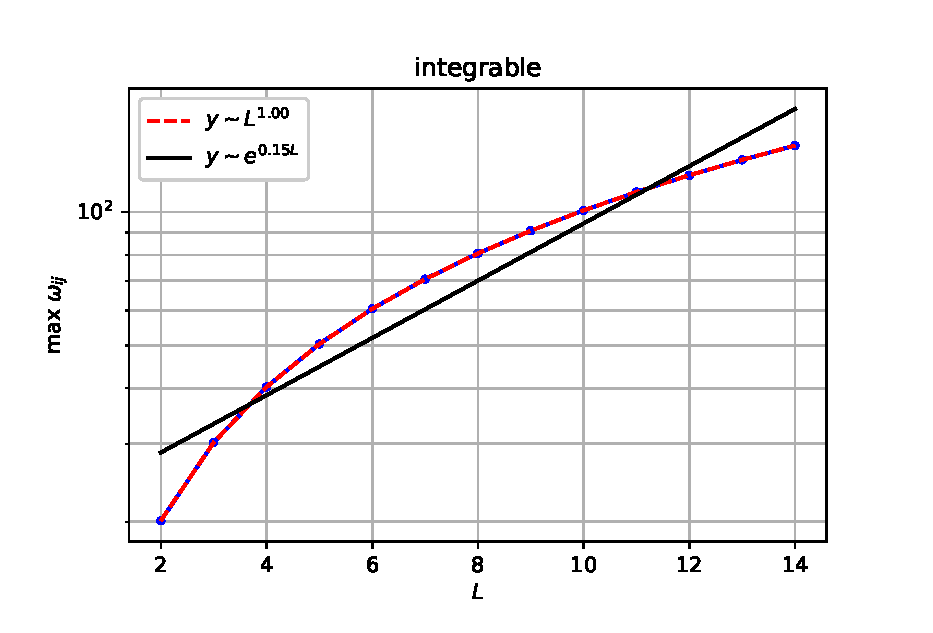
\includegraphics[scale=0.53]{new_pics/v2_maxwij_int.eps}
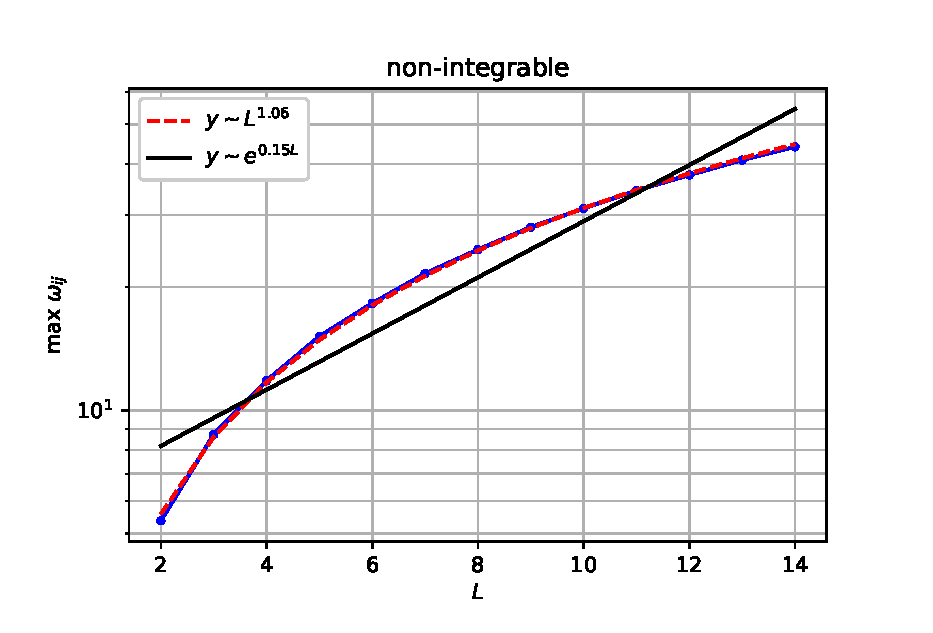
\includegraphics[scale=0.53]{new_pics/v2_maxwij_nonint.eps}
\caption{Using ED method, $\min \omega_{ij}(L)$}
\end{center}
\end{figure}



If there is degeneracy, $\min \omega_{ij}(L)$ should be zero. Why don't I see any degenerate level?

I find that because of open boundary conditions, I don't get any degenerate states for integrable model\footnote{Can I see this analytically for a simple model with only $J \sum_i\sigma_{i+1}^z \sigma_{i}^z$ term?}. The question is then how do I get an almost linear scaling of norm for integrable models? We had reasoned that $\langle n| \partial_{\lambda} H|m\rangle$ is zero because of extensive number of degenerate levels. It doesn't seem like that here.


\begin{figure}[!ht]
\begin{center}
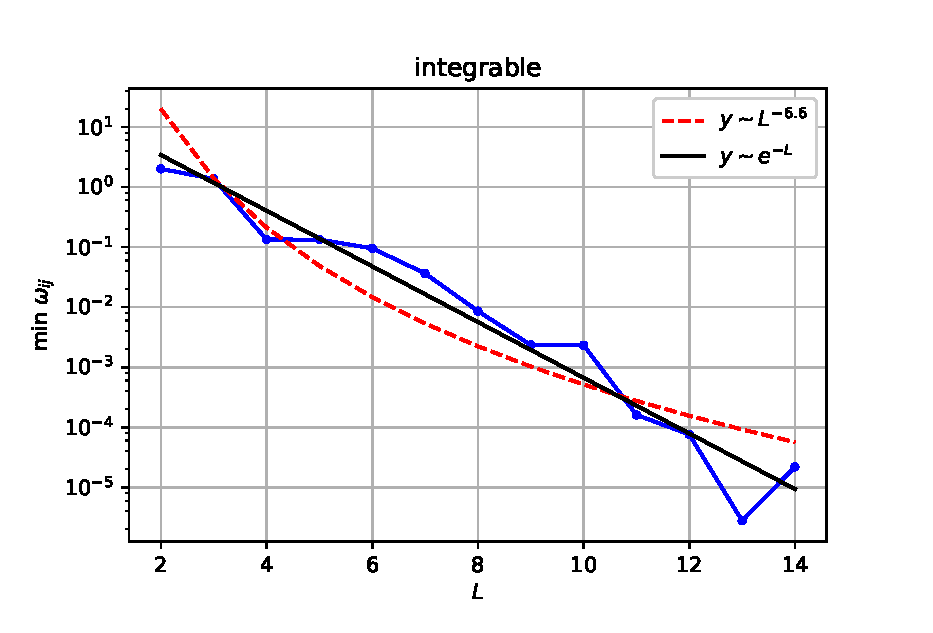
\includegraphics[scale=0.535]{new_pics/v2_minwij_int.eps}
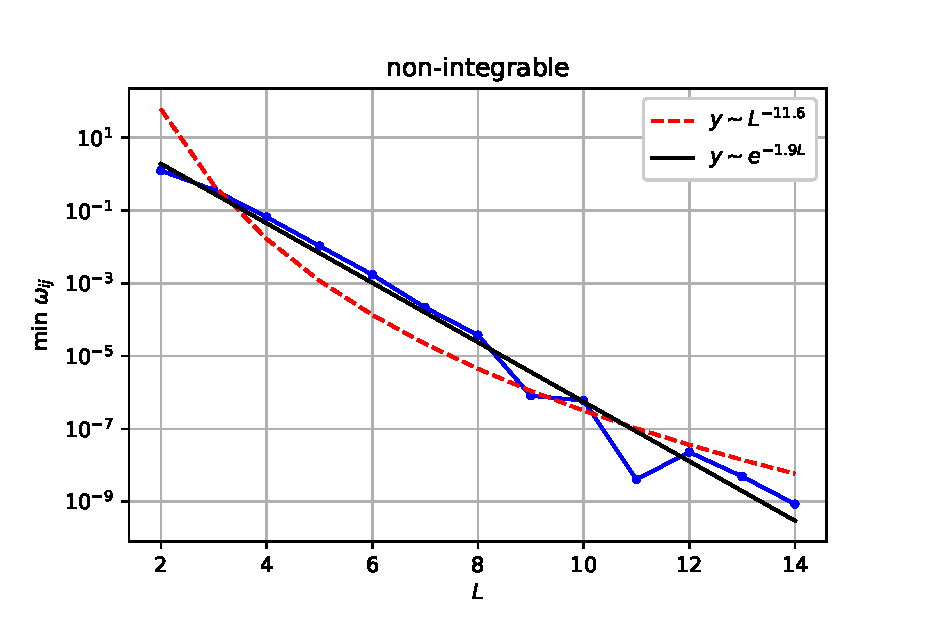
\includegraphics[scale=0.535]{new_pics/v2_minwij_nonint.eps}
\caption{Using ED method,  $\max \omega_{ij}(L)$}
\end{center}
\end{figure}


\section{Norm computed using ED}

Let's look at the expression of off-diagonal elements of gauge potential:
\begin{equation}
\langle m |A_{\lambda} | n \rangle =  -i \hbar \dfrac{\langle m |\partial_{\lambda}H | n \rangle}{E_m-E_n}, \quad n \neq m
\end{equation}
We see that while using ED, we need to be wary of degenerate eigenvalues. Do these degenerate eigenvalues contribute to norm of gauge potential? Answer is no because $\langle m |\partial_{\lambda}H | n \rangle=0$ for degenerate pair of eigenvalues as shown in appendix \ref{sec.deg}.



%We have two options while computing norm using ED: either take out all degenerate eigenvalues and work in non-degenerate eigen-subspace or introduce a cutoff $\mu$ to help us out here. We find that second option is easier to work numerically. Our $\mu$-dependent gauge potential is given by:
%\begin{equation}
%\langle m |A_{\lambda} | n \rangle =  -i \hbar \dfrac{\langle m |\partial_{\lambda}H | n \rangle}{\omega_{mn}^2+ \mu^2} \omega_{mn}
%\end{equation}
%We note that for $\mu \neq 0$, $A_{\lambda}$ is zero for degenerate levels $n$ and $m$. What should be the value of $\mu$ chosen?  If $\mu^2 \ll \omega_{mn}^2$, then we would be back to square one because then we can ignore $\mu^2$ in denominator, and then the computer would complain of division by zero problem for degenerate levels $n$ and $m$. If $\mu^2 \gg \omega_{mn}^2$, then we would get approximate gauge potential, not the exact one. Numerically, we choose $\mu^2$ to be the difference between two closest floating point numbers.

%We would be studying integrable model, and seeing how norm of gauge potential scales.
%\begin{equation}
%H= -J \sum_{j} \sigma_j^x(\sigma_{j+1}^x+ \sigma_{j-1}^x) - \lambda \sum_{j} \sigma_j^z 
%\end{equation}
%where we have chosen $J=1$ and $\lambda=5$ with open boundary conditions.
%
%\begin{equation}
%H= -J \sum_{j} \sigma_j^x (\sigma_{j+1}^x+ \sigma_{j-1}^x) - h\sum_{j} \sigma_j^z -\lambda \sum_{j} \sigma_j^x 
%\end{equation}
%where we have chosen $J=1$, $h= (\sqrt{5}+1)/4$ and $\lambda=(\sqrt{5}+5)/8$ with open boundary conditions.


%\begin{figure}
%\begin{center}
%%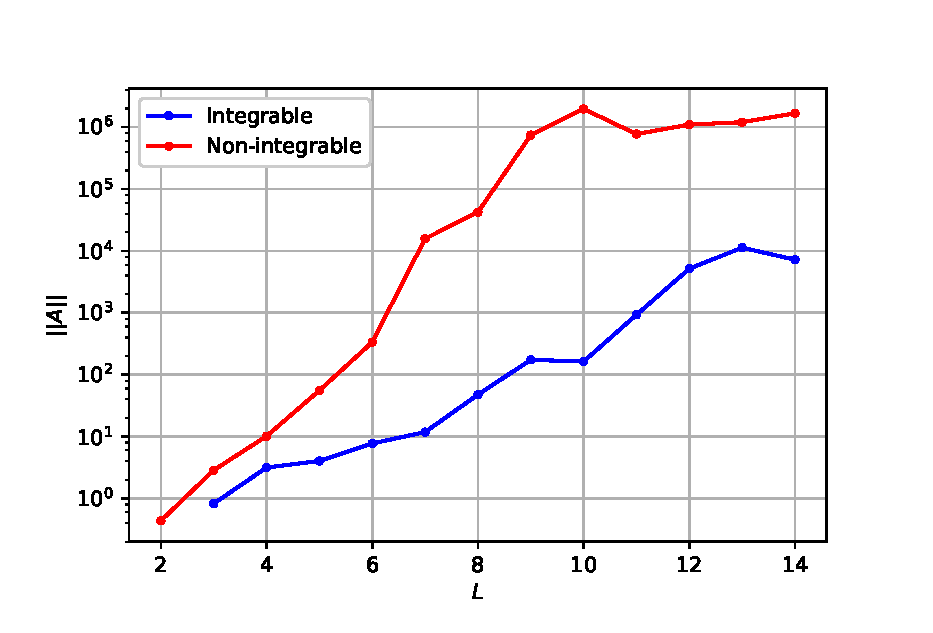
\includegraphics[scale=0.65]{norm.eps}\\
%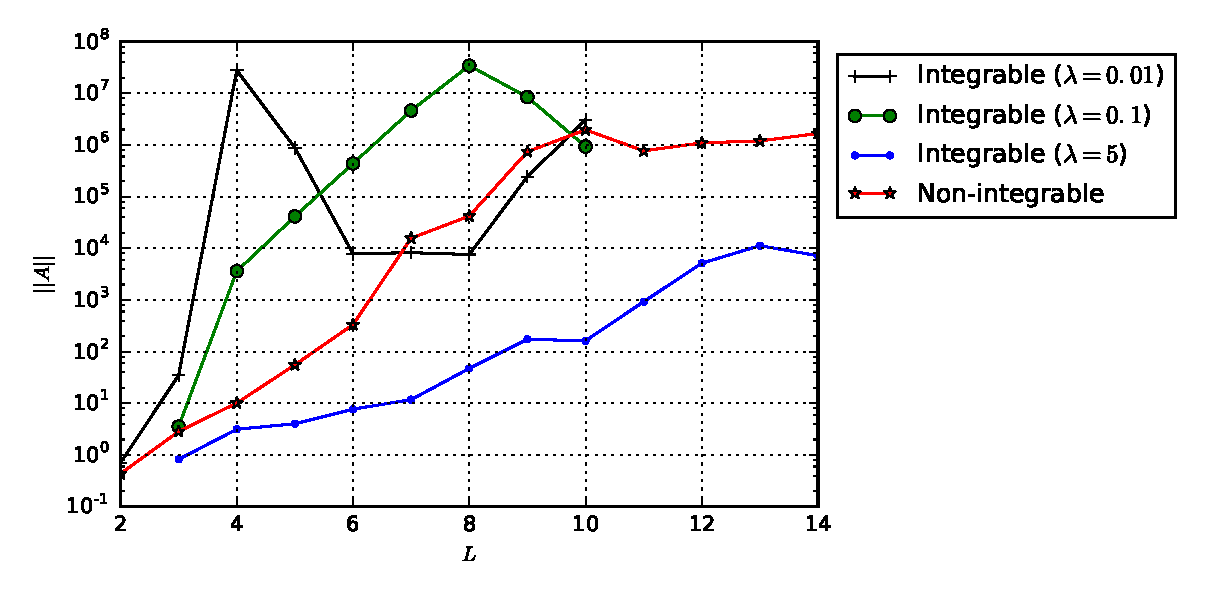
\includegraphics[scale=0.65]{norm_integ.eps}
%\caption{System size (L) scaling of norm of gauge potential in integrable and non-integrable systems}
%\end{center}
%\end{figure}
%
%
%\begin{figure}
%\begin{center}
%%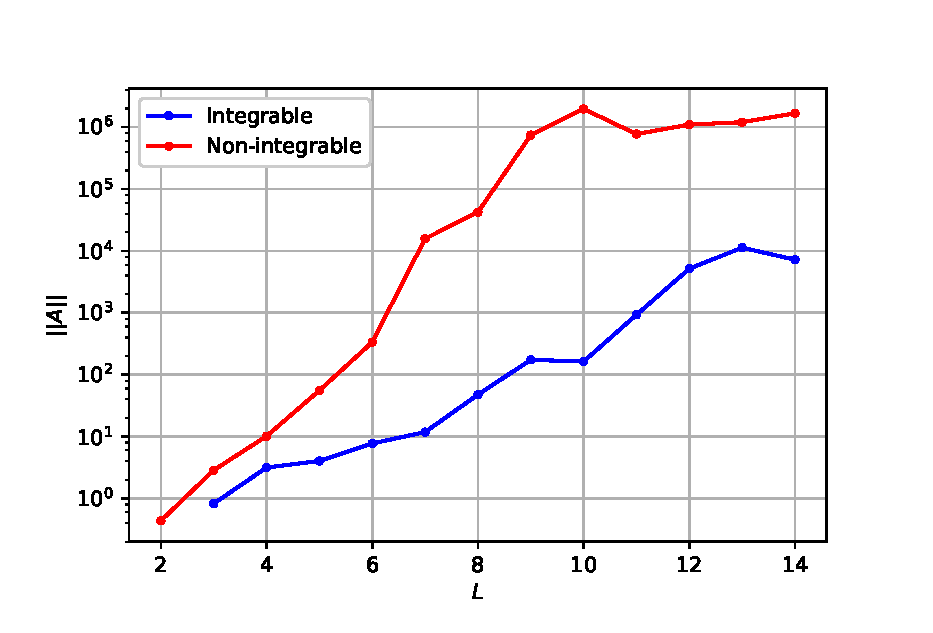
\includegraphics[scale=0.65]{norm.eps}\\
%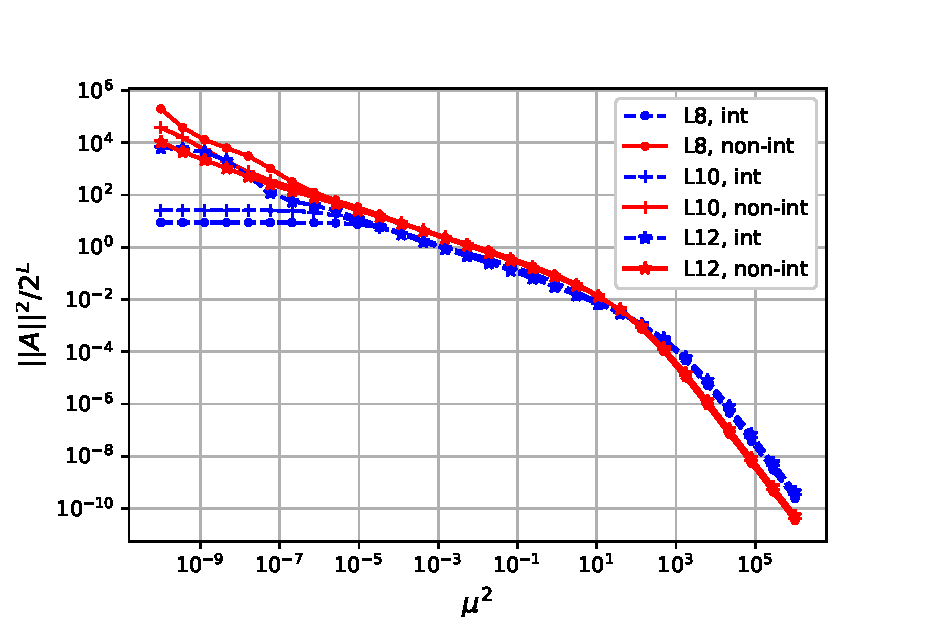
\includegraphics[scale=0.65]{norm_mu_scaling_all_L.eps}
%\caption{$\mu$ scaling of norm of gauge potential in integrable and non-integrable systems}
%\end{center}
%\end{figure}
%
%
%
%\begin{figure}
%\begin{center}
%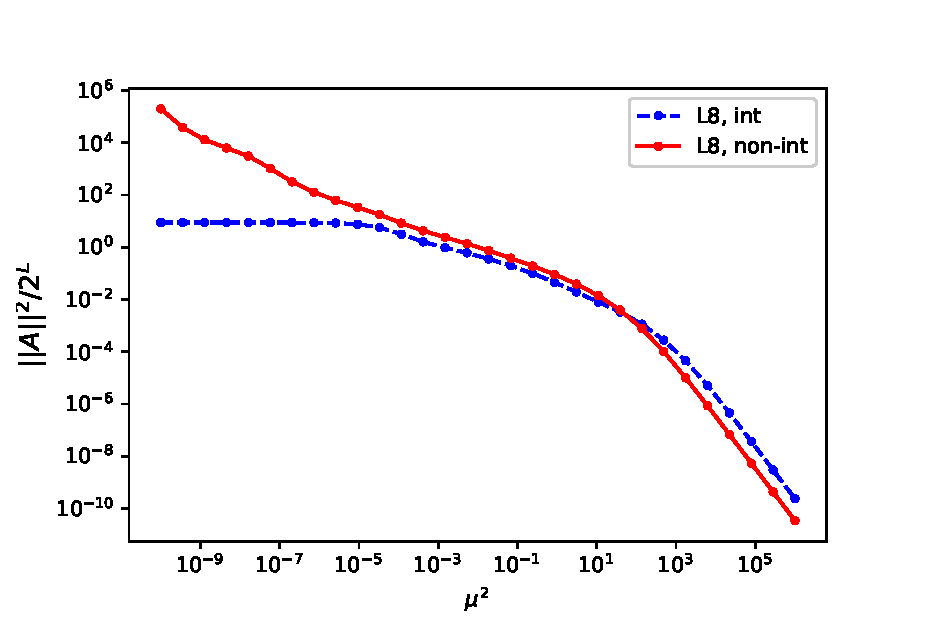
\includegraphics[scale=0.53]{norm_mu_scaling_L8.eps}
%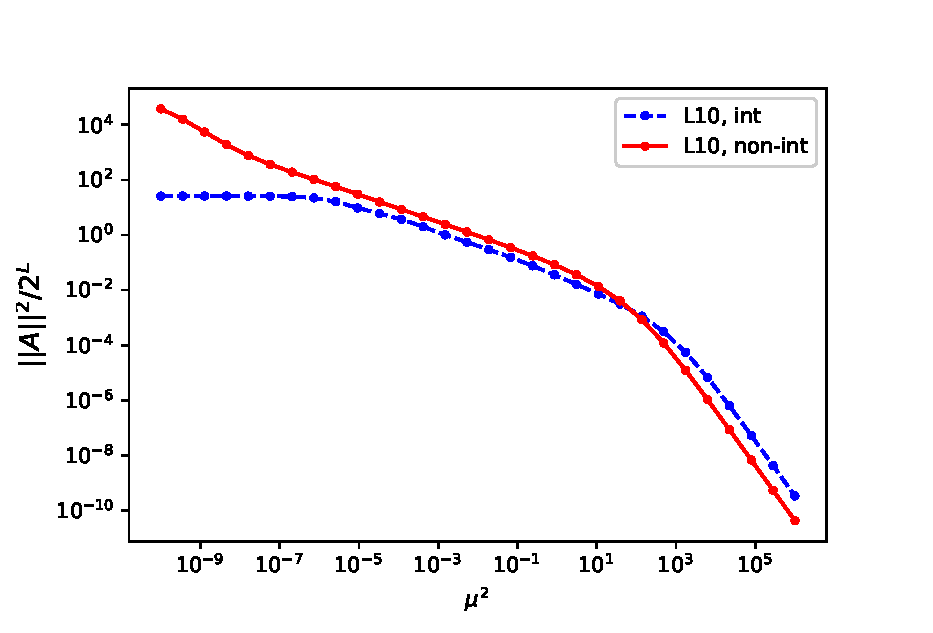
\includegraphics[scale=0.53]{norm_mu_scaling_L10.eps}\\
%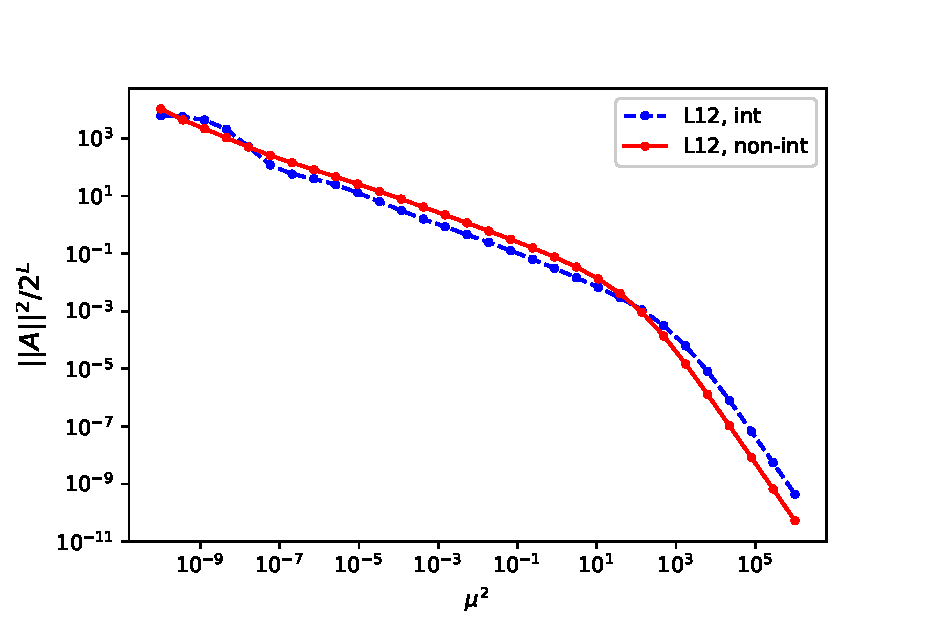
\includegraphics[scale=0.67]{norm_mu_scaling_L12.eps}
%\caption{$\mu$ scaling of norm of gauge potential in integrable and non-integrable systems}
%\end{center}
%\end{figure}

For integrable model, we would study the Hamiltonian of Transverse Field Ising model:
%\begin{equation}
%H= J \sum_{j} \sigma_j^z(\sigma_{j+1}^z+ \sigma_{j-1}^x) + \lambda \sum_{j} \sigma_j^z 
%\end{equation}

%and this:
\begin{equation}
H= J \sum_{j=1}^{L-1} \sigma_j^z \sigma_{j+1}^z + \lambda \sum_{j} \sigma_j^x
\end{equation}

%\begin{equation}
%H= J \sum_{j=1}^L-1 \sigma_j^z(\sigma_{j+1}^z+ \sigma_{j-1}^z) + \lambda \sum_{j} \sigma_j^x
%\end{equation}

where we have chosen $J=1$ and $\lambda=5$ with open boundary conditions.

For non-integrable model, we would study the Hamiltonian of Ising model with both transverse and longitudinal fields:
\begin{equation}
H= J \sum_{j=1}^{L-1} \sigma_j^z \sigma_{j+1}^z + h\sum_{j} \sigma_j^z +\lambda \sum_{j} \sigma_j^x 
\end{equation}
%
%\begin{equation}
%H= J \sum_{j} \sigma_j^z (\sigma_{j+1}^z+ \sigma_{j-1}^z) + h\sum_{j} \sigma_j^z +\lambda \sum_{j} \sigma_j^x 
%\end{equation}
where we have chosen $J=1$, $h= (\sqrt{5}+1)/4$ and $\lambda=(\sqrt{5}+5)/8$ with open boundary conditions. These are values of parameters for which this model has been shown to be robustly non-integrable for small systems \cite{kim2013ballistic}.

We see that $\partial_{\lambda}H =  \sum_{j} \sigma_j^x  $.

Since anti-ferromagnetic phase has more local order compared to ferromagnetic phase, we expect the former to be less affected by finite size effects.





\subsection{$\mu$ scaling of gauge potential}



\begin{figure}[!ht]
\begin{center}
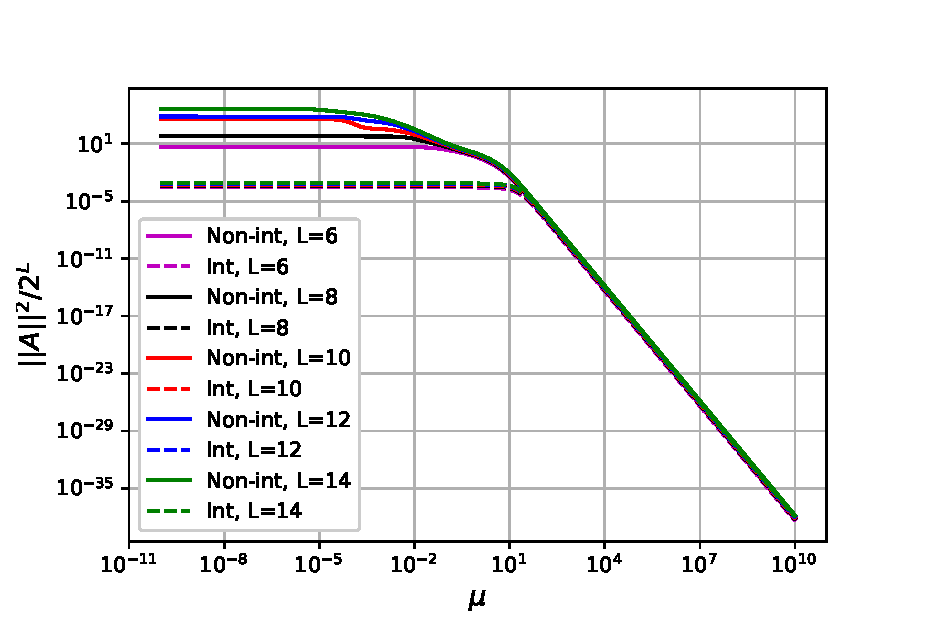
\includegraphics[scale=0.51]{new_pics/v2_norm_mu_scaling.eps} 
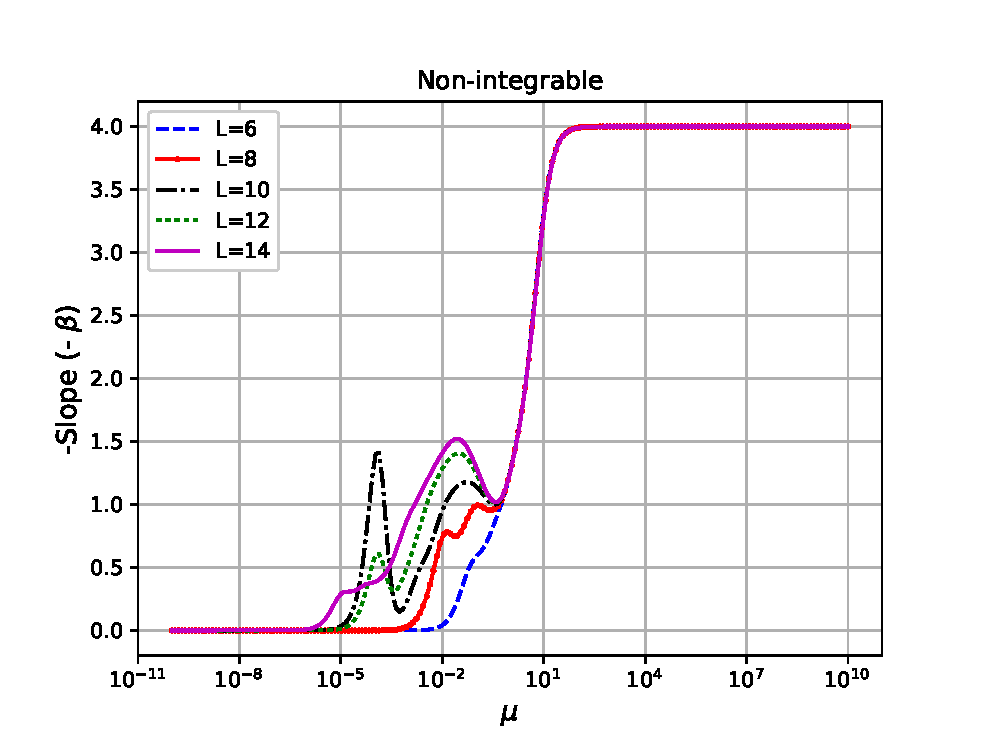
\includegraphics[scale=0.43]{new_pics/v3_slope_nonint_semilogx.eps}
%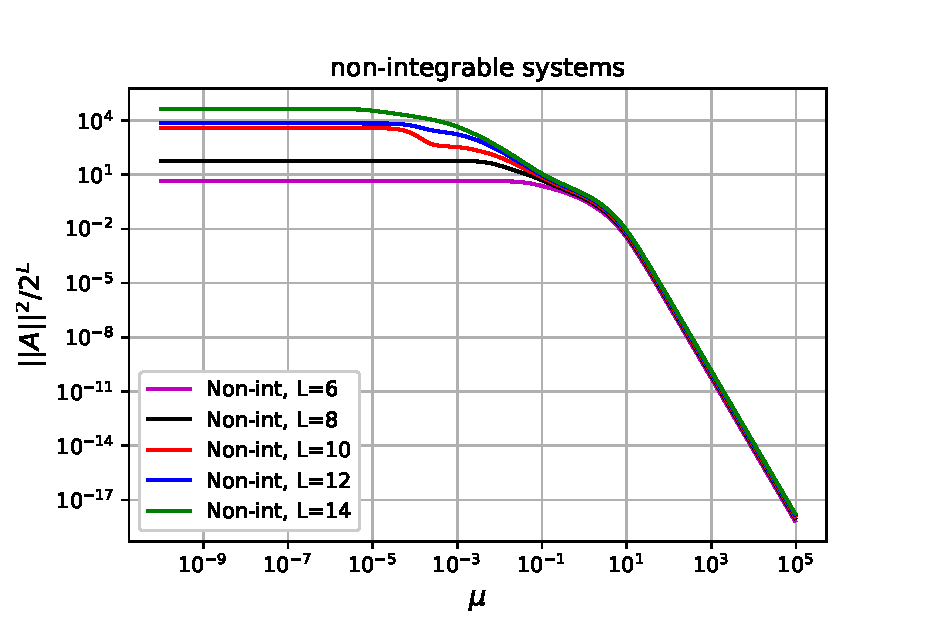
\includegraphics[scale=0.7]{new_pics/v2_norm_mu_scaling_nonint.eps}
\caption{a) Using ED method, we obtain  $\mu$ dependence of norm of gauge potential in integrable and non-integrable systems b) $\mu$ dependence of negative of slope ($-\beta (\mu)$) is shown for non-integrable systems}
\label{mu_scaling}
\end{center}
\end{figure}


Our $\mu$-dependent gauge potential $A_{\lambda}$ is given by:
\begin{equation}
\langle m |A_{\lambda} | n \rangle =  -i \hbar \dfrac{\langle m |\partial_{\lambda}H | n \rangle}{\omega_{mn}^2+ \mu^2} \omega_{mn}
\end{equation}
where $\omega_{nm}=E_n-E_m$ and eigenstates depend on $\lambda$, i.e.$|n \rangle= |n (\lambda) \rangle $. Hence, norm should be (in units of $\hbar=1$):
\begin{equation}
||A_{\lambda}||^2 = \sum_n \sum_{m \neq n}  \dfrac{\omega_{nm}^2}{(\omega_{nm}^2 + \mu^2)^2} |\langle m | \partial_{\lambda}H| n \rangle|^2
\end{equation}

Numerically, we find the dependence of gauge potential on $\mu$ using Exact Diagonalization method (ED) in figure \ref{mu_scaling}. Let's claim that $||A||^2/2^L=\alpha\mu^{\beta}$. Then if we take log both sides, we get
\begin{equation}
\log ||A||^2/2^L=\log \alpha+ \beta \log \mu
\end{equation}
where $\beta$ is the slope on a log-log scale. Numerically, we can find $\beta_i$ for each pair of points using the following relationship (figure \ref{mu_scaling}):
\begin{equation}
\beta_i=\dfrac{\log y( \mu_{i+1}) -\log y( \mu_{i})} {\log \mu_{i+1}-\log \mu_{i}}
\end{equation}
where $y= ||A||^2/2^L$. 
%\begin{figure}[!ht]
%\begin{center}
%%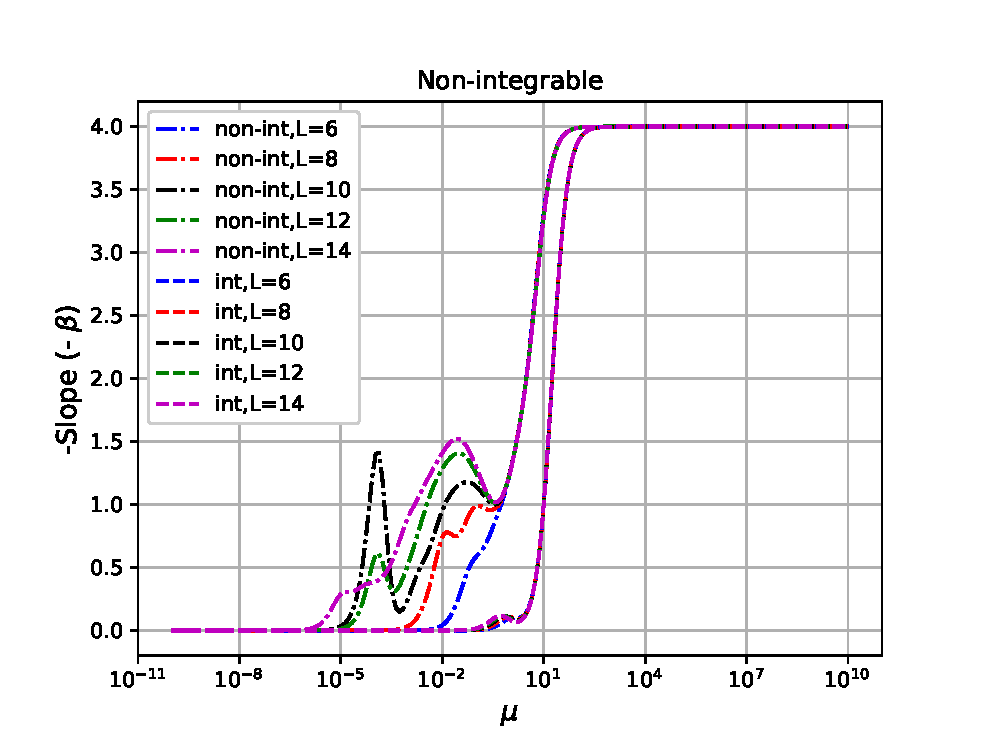
\includegraphics[scale=0.7]{new_pics/v3_slope_nonint_int_compare_semilogx.eps}\\
%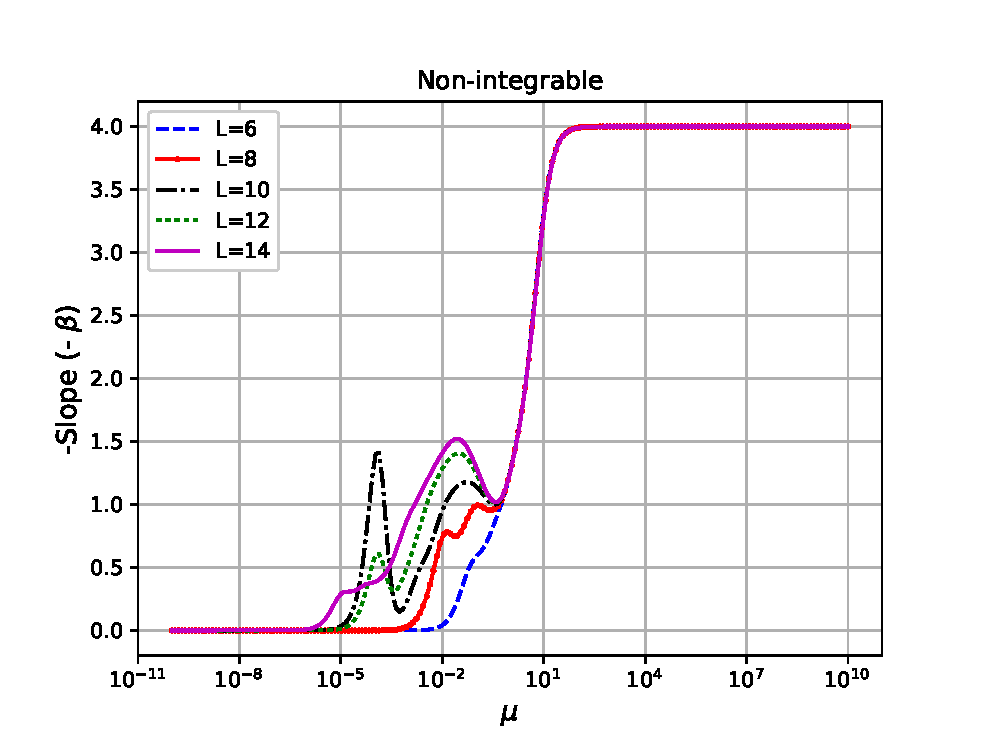
\includegraphics[scale=0.7]{new_pics/v3_slope_nonint_semilogx.eps}
%\caption{$\mu$ dependence of negative of slope ($-\beta (\mu)$) is shown for non-integrable systems }
%%\label{slope_nonintegrable_mu}
%\end{center}
%\end{figure}








%Let's stick to non-integrable systems for now%(figure \ref{nonintegrable_mu}).

%\begin{figure}[!ht]
%\begin{center}
%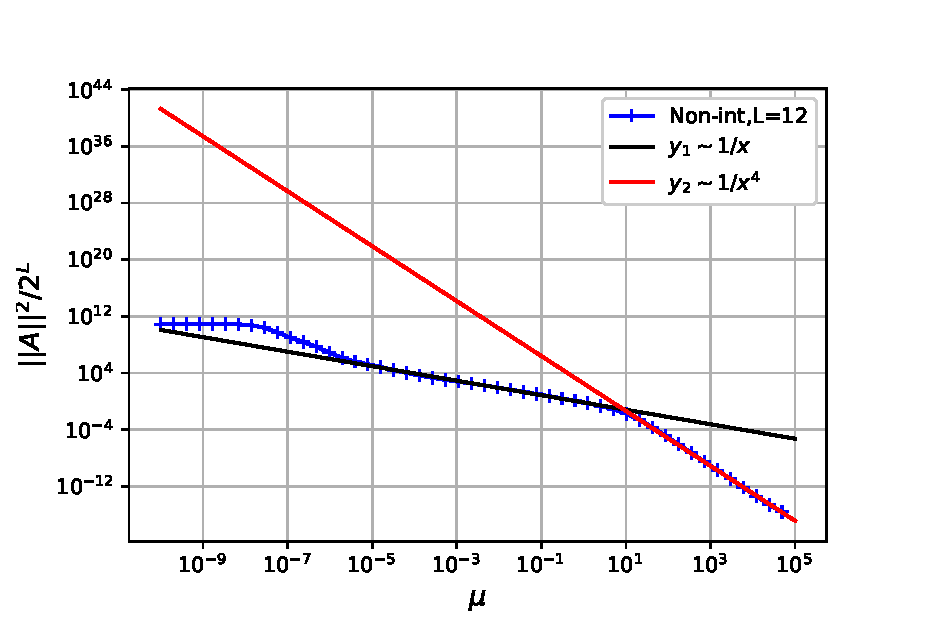
\includegraphics[scale=0.7]{L12_two_scaling.eps}
%\caption{Two different scaling regimes of $1/\mu$ and $1/\mu^4$: $y_1=\alpha_1\mu^{\beta_1}$ and $y_2=\alpha_2\mu^{\beta_2}$ where $\beta_1=-1.02$, $\beta_2=-3.88$, $\alpha_1=0.682$ and $\alpha_2=328.38$ which are found using least square method. $\min\{w_{nm}\}=2.31\times10^{-8}$ and $\max\{w_{nm}\}=37.58$ }
%\label{nonintegrable_mu}
%\end{center}
%\end{figure}

 Let's study two regimes we see in the figures: 
\begin{itemize}
\item \textbf{Constant in $\mu$ regime} when $\mu \ll \min\{w_{nm}\}$: Since density of states is highest in the middle of spectrum, $\min\{w_{nm}\}$ is smallest for two states lying there. In this regime, $\mu$ is so small that it doesn't really affect the norm of gauge potential. So, we get exact gauge potential in this regime.
\begin{equation}
||A_{\lambda}||^2 = \sum_n \sum_{m \neq n}  \dfrac{|\langle m | \partial_{\lambda}H| n \rangle|^2}{\omega_{nm}^2}  \sim 2^Le^L
\end{equation}
This regime seems to grow smaller for larger system size (figure \ref{mu_scaling}).

\begin{figure}[!ht]
\begin{center}
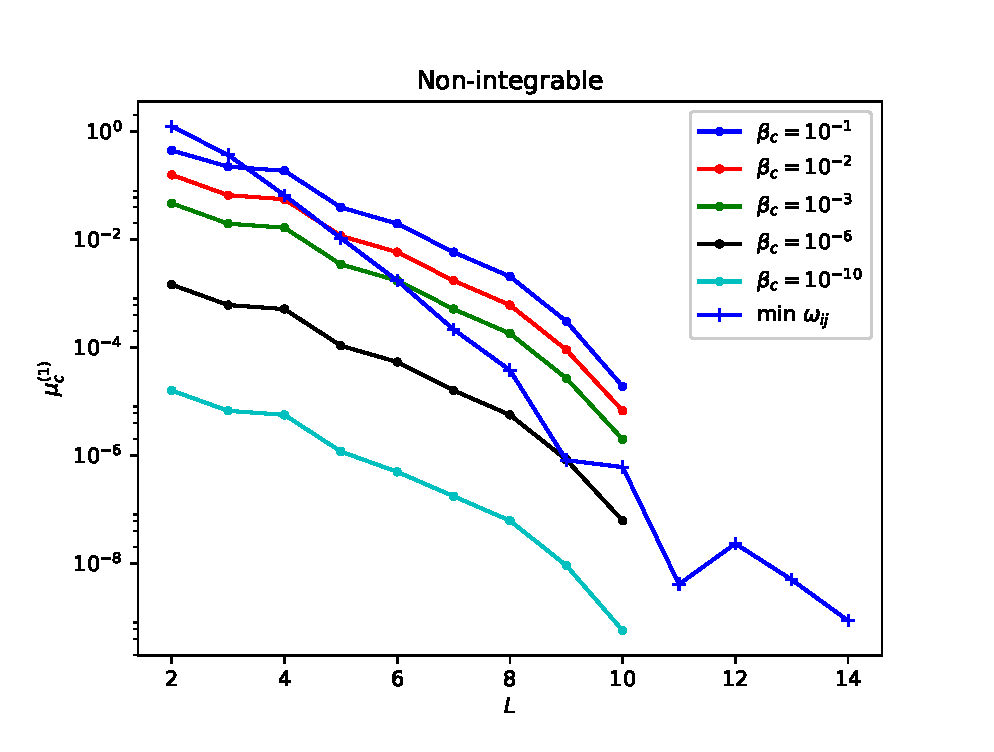
\includegraphics[scale=0.5]{new_pics/mu_c_1_nonint.eps}
\caption{$\mu_c^{(1)}$ dependence of system size L }
%\label{slope_nonintegrable_mu}
\end{center}
\end{figure}



%\begin{figure}[!ht]
%\begin{center}
%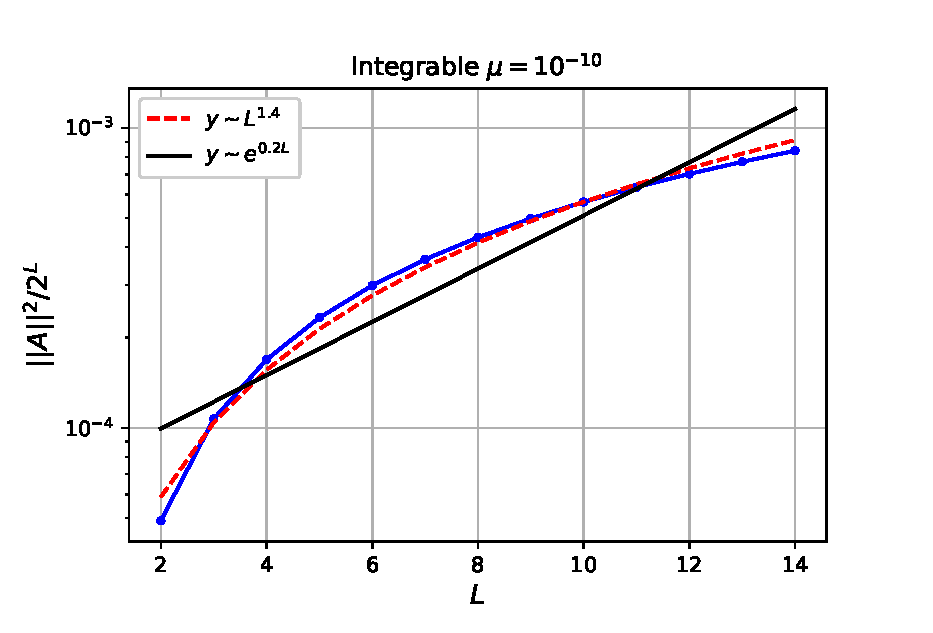
\includegraphics[scale=0.7]{new_pics/v2_int_exactgauge_Lscaling.eps}
%%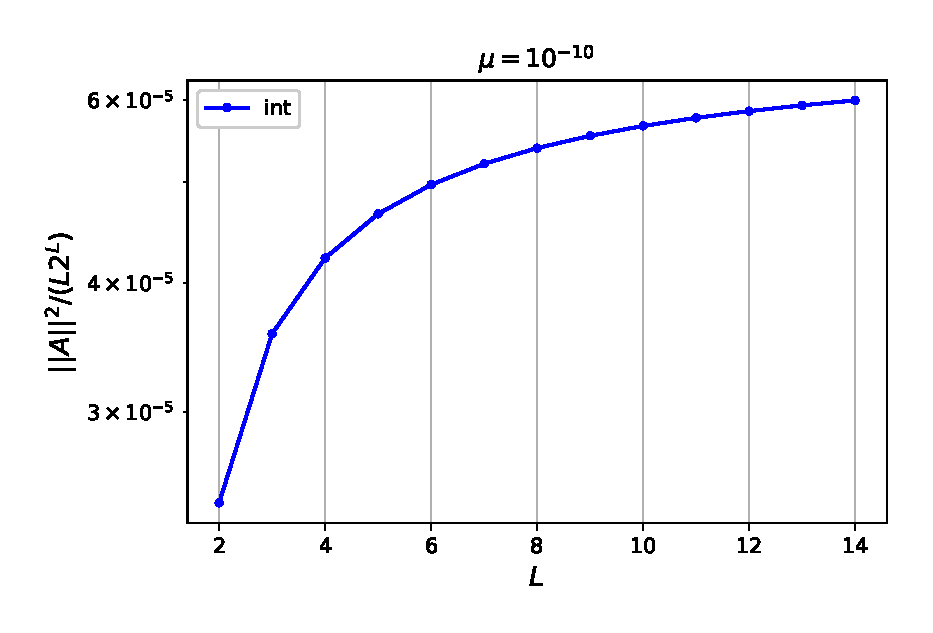
\includegraphics[scale=0.7]{new_pics/v2_1_norm_int_linear.eps}
%\caption{Integrable systems: exact gauge potential as a function of system size with open boundary conditions. Periodic boundary conditions shows linear scaling in system size. }
%\end{center}
%\end{figure}



\item \textbf{$1/\mu^4$ scaling regime} 
When $\mu \gg \max\{w_{nm}\}$, approximate gauge potential $A_{\lambda}^*$ would be given by:
\begin{align*}
A_{\lambda}^* & =  -i \hbar [H,\partial_{\lambda}H ]\dfrac{1}{\mu^2}  \\
& =  -i \hbar \dfrac{1}{\mu^2} C^{(1)}
\end{align*}
where $ C^{(1)}=2i \left(\sum_{j=1}^{L-1} \sigma_j^y \sigma_{j+1}^z + \sum_{j=2}^{L} \sigma_j^y \sigma_{j-1}^z + h \sum_{j=1}^{L}\sigma_j^y \right) $.


\begin{align*}
||A_{\lambda}||^2 &=\dfrac{\alpha_2^{Th}}{ \mu^4} \sim\dfrac{L}{ \mu^4} 2^L 
% \dfrac{1}{ \mu^4} \sum_n \sum_{m \neq n}  \omega_{nm}^2 |\langle m | \partial_{\lambda}H| n \rangle|^2 = \dfrac{1}{ \mu^4} \Tr  [H, \partial_{\lambda}H]^2
\end{align*}

where theoretical value of  $\alpha_2^{Th}=\Tr  [H, \partial_{\lambda}H]^2 $ should be compared against the numerical value obtained in figure.  For $L=12$, we obtain $\alpha_2^{Th}=119.41$ whose details are given in appendix B.


What is really interesting here in this regime is that approximate gauge potential has only a single body term and a two body term. In other words, when comparing it with exact gauge potential which has $C^{(1)},C^{(3)}, C^{(5)} $ terms involving all many body operators, we have only two and one body term here.

%\item \textbf{Intermediate regime of $1/\mu$ scaling:} For non-integrable systems, we can use ETH to claim that after assuming $f_O$ doesn't depend on $\omega$:
%\begin{equation}
%\dfrac{||A_{\lambda}||^2}{2^L}= \dfrac{\pi }{4 \mu} \langle |f_O(E_n)|^2  \rangle \sim \dfrac{L^\gamma }{ \mu} 
%\end{equation}
%where $\gamma$ is unknown. Probably $\gamma$  depends on $\mu$.
\end{itemize}

\subsection{L scaling of gauge potential}
\begin{figure}[!ht]
\begin{center}
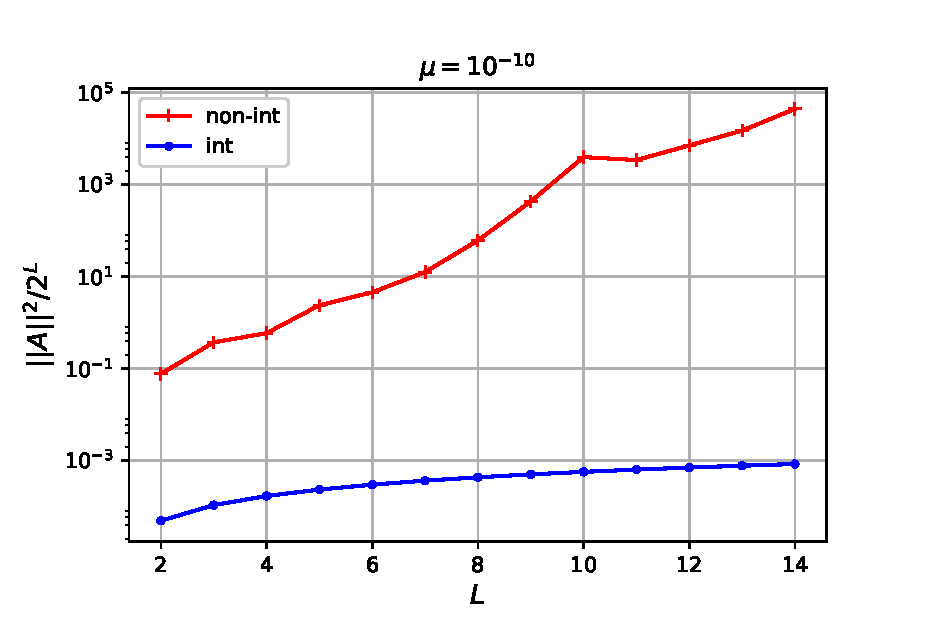
\includegraphics[scale=0.7]{new_pics/v2_1_norm_L_scaling.eps}
\caption{Exact gauge potential as a function of system size: non-integrable systems (exponential scaling) and integrable (polynomial scaling) }
\end{center}
\end{figure}

%\underline{\textit{A few comments here:}}

%\item It's very interesting that there are only two ``kinds" of approximate gauge potential regimes -- the $1/\mu$ regime which is polynomial ($L^{\gamma}$) in the system size and the $1/\mu^4$ regime which is linear in the system size \footnote{Of course, I am ignoring the regime which is between the regime of exact gauge potential (constant plateau regime) and $1/\mu$ scaling. It can't be described using one single exponent $\beta$ unlike three other regimes-- $\beta=0, -1, -4$}. 
%
%In $1/\mu^4$ regime, we know definitely that only two and one body terms survive. In $1/\mu$ regime, which operators survive and which don't? Why there are only two ``kinds" of approximate gauge potential when we introduce a cutoff in our theory? In other words, since exact gauge potential has all possible many body terms for nonintegrable model, we expect that when we introduce $\mu$, magnitude of these terms should be smaller (but all should be still there). Probably in $1/ \mu$ regime all these terms are there unless $\gamma =1/2$. Question is why suddenly at second critical $\mu_c$, we find that approximate gauge potential becomes linear (only single and two body) in system size?
% \textbf{Checks on my numerical results:}
%\begin{itemize}
%%\item Numerically, go for smaller systems and see if this pattern is seen there too or not. If that's happening, we can probably verify it in the analytical calculations.
%%\item Analytically using cutoff regulator formula,  check N=2 and N=4 and verify if these two regimes show up. How does the operators look like for $1/\mu$ scale?
%%\item $\mu_c^{(1)} \sim \min{\omega_{nm}}$ $\mu_c^{(2)} \sim \max{\omega_{nm}}$. It should be same order of magnitude.
%\end{itemize}
%For integrable model, I don't know how to explain $1/\mu$ scaling.

\appendix
\section{Do degenerate eigenvalues contribute to norm of gauge potential?}\label{sec.deg}
Let's consider $H | n(\lambda) \rangle= E_n  | n(\lambda) \rangle $. Hence, we have $\langle m(\lambda)  |  H | n(\lambda) \rangle=0$ for $n\neq m$. We can exploit this property to get some insight:
\begin{align*}
\partial_{\lambda}\langle m  |  H | n\rangle&=0\\
\langle \partial_{\lambda} m |  H | n \rangle + \langle  m  |  H |\partial_{\lambda} n \rangle + \langle  m  | \partial_{\lambda} H | n \rangle&=0\\
\langle \partial_{\lambda} m   | n \rangle E_n + E_m\langle  m  |   \partial_{\lambda} n \rangle + \langle  m  | \partial_{\lambda} H | n \rangle&=0\\
(E_n - E_m)\langle  \partial_{\lambda} m  |    n \rangle + \langle  m  | \partial_{\lambda} H | n \rangle&=0
\end{align*}

Hence, we find that if there are two degenerate energy levels $n$ and $m$ such that $E_n=E_m$, then $\langle  m  | \partial_{\lambda} H | n \rangle=0$. Hence, the contribution to norm of gauge potential from this pair of energy levels will be zero. I should check this numerically if results of my code respect this property.


\section{Computing $\Tr [H, \partial_{\lambda}H] $}
\subsection{Integrable model}
\begin{equation}
H=  \sum_{j=1}^{L-1} \sigma_j^z \sigma_{j+1}^z + \lambda \sum_{j} \sigma_j^x
\end{equation}
We know that that $\partial_{\lambda}H =  \sum_{j} \sigma_j^x $. Let's denote  $C^{(1)}=[H,\partial_{\lambda}H]$. 


\begin{align*}
[H,\partial_{\lambda}H] & = \sum_{j=1}^{L-1} [\sigma_j^z \sigma_{j+1}^z , \sum_{i} \sigma_i^x]  \\
&= 2i \left(\sum_{j=1}^{L-1} \sigma_j^y \sigma_{j+1}^z + \sum_{j=2}^{L} \sigma_j^y \sigma_{j-1}^z\right)
\end{align*}

We find that $\Tr |C^{(1)}|^2 = 8 (L-1)2^L$ 

\subsection{Non-integrable model}
Non-integrable model's Hamiltonian is given by: 
\begin{equation}
H= J \sum_{j=1}^{L-1} \sigma_j^z \sigma_{j+1}^z + h\sum_{j} \sigma_j^z +\lambda \sum_{j} \sigma_j^x 
\end{equation}
\begin{align*}
[H,\partial_{\lambda}H] & =  [\sum_{j=1}^{L-1} \sigma_j^z \sigma_{j+1}^z + h\sum_{j=1}^{L} \sigma_j^z, \sum_{i} \sigma_i^x]  \\
&= 2i \left(\sum_{j=1}^{L-1} \sigma_j^y \sigma_{j+1}^z + \sum_{j=2}^{L} \sigma_j^y \sigma_{j-1}^z + h \sum_{j=1}^{L}\sigma_j^y \right) 
\end{align*}


We find that $\Tr |C^{(1)}|^2 = 2^L 4(h^2 L + 2J(L-1))$ 



\subsection{Integrable systems with open boundary condition}

\begin{figure}[!ht]
\begin{center}
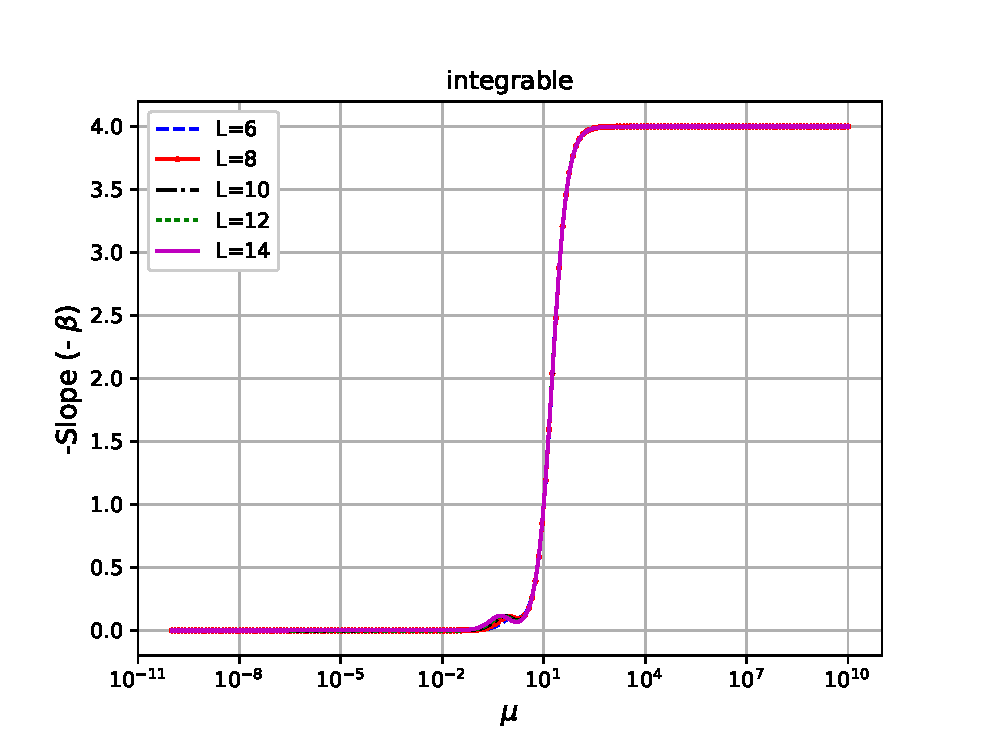
\includegraphics[scale=0.5]{new_pics/v3_slope_int_semilogx.eps} 
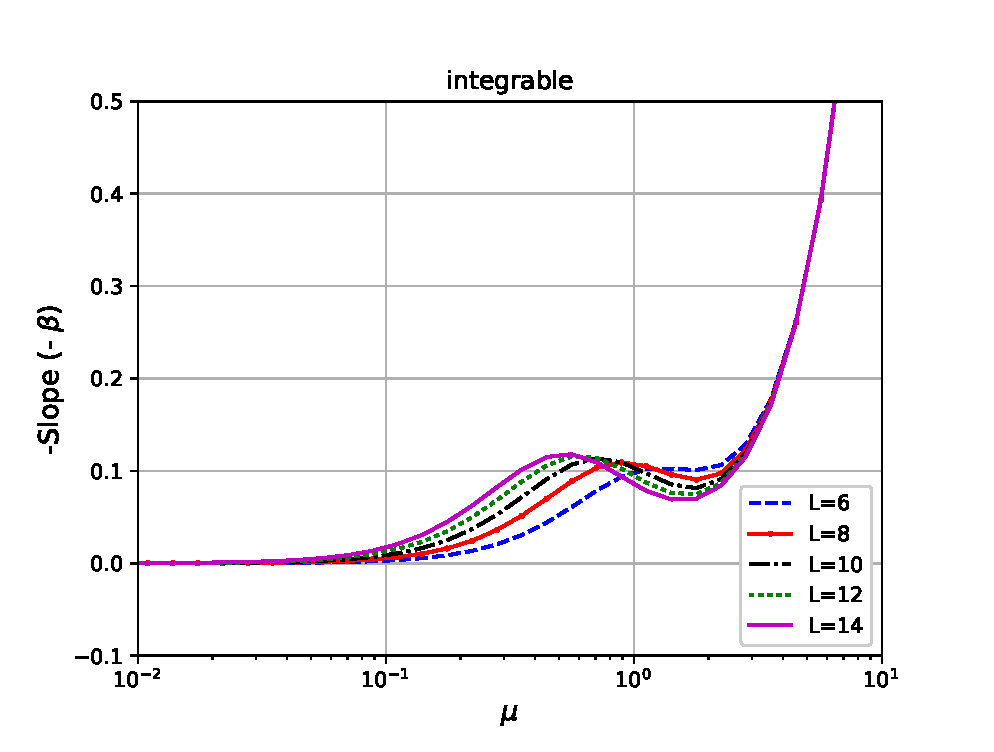
\includegraphics[scale=0.5]{new_pics/v3_slope_int_semilogx_zoom.eps}
\caption{$\mu$ dependence of negative of slope ($-\beta (\mu)$) is shown for  integrable systems }
\label{slope_integrable_mu}
\end{center}
\end{figure}

\bibliography{ref} 

\bibliographystyle{unsrt}
%\bibliographystyle{plain}

\end{document}
